\documentclass[12pt,twocolumn]{article}
\usepackage[margin=0.7in]{geometry}
\usepackage{graphicx}
\usepackage{cite}
                                        
%%%%%%%%%%%%%%%%%%%%%%%%%%%%%%%%%%%%%%%%%%%%%%%%%%%%%%%%%%%%%%%%%%%%%%%%%%%%%%%%%%%%%%%%%%%%%%%%%%%%%%%%%%%%%%%%%%%%%%%%%%%%%%%%%%%%%%%%%%%%%%%%%%%%%%%%%%%%%%%%%%%%%%%%%%%%%%%%%%%%%%%%%%%%%%%%%%%%%%%%
                                        
\begin{document}
\title{A Study of the Energy Quantization in Atomic Structure}
\author{Joseph Hartsell and M. Lane}
\date{\today}

\maketitle


\begin{abstract}
	In this lab two different gasses are used in a Franck-Hertz type experiment to observe quantization within atomic structure. Measure current through mercury vapor as a function of electron energy and calculated the first excitation of mercury to be at 4.7eV. Using the same procedure with Helium gas, we found excitation levels of Helium. In the third part of this experiment, we observed helium and mercury spectrum emissions and used the emissions to calculate a diffraction grating spacing and the transition levels for helium.
\end{abstract}

\section{Introduction}

Physics of the early twentieth centry is characterized almost entirely by quantum effects, and the first experiment to truly witness quantization was the Frack-Hertz experiment. The idea of quantization began with Max Planck's solution to the Ultraviolet Catastrophe in 1900 followed by Einstein's explanation of the photoelectric effect. Together these two experiments brought quantization to light. In 1909 Rutherford introduced a new model of the atom and in 1913 Neils Bohr expanded on the model and introduced quantized energy levels to the atom.

Bohr's model of the atom was groundbreaking and his calculations unraveled the mystery behind the Rydberg formula and the Hydrogen spectrum. However, the model broke down for other elements and had yet to be experimentally verified. In 1914 James Franck and Gustav Hertz developed an elegantly simple experiment to verify the Bohr model and its proposed energy levels. They began with an emission spectrum whose distinct lines clearly indicated quantization. The problem with standard emission spectrums is the lack of control over the process. There are no restrictions on the electrons exciting the system resultng in every excitation and relaxation taking place. While the bands displayed agree with Bohr's model, it is insufficient proof of quantization since the excitations and relaxations are not directly witnessed.

Franck and Hertz addressed this issue by using a controlled electron gun to inject into the vapor only electrons of a specific kinetic energy. These electrons were fired through a vapor where they either were absorbed and reemitted with less kinetic energy or passed through without interacting. By adding a second retarding potential and collector plate after the vapor, the reemitted low-energy electrons could be distinguished from the high electrons. If Bohr's model was correct, they predicted that current registered on the collector plate would increase as accelerating voltage increased, implying the electrons do not in general interact with the gas. However, when a certain accelerating voltage is reached, the Bohr model allows interactions and the current should suddenly and drastically drop.

In this lab, we will reconstruct two variations of this experiment using mercury vapor and helium vapor. We will also examine the emission spectrum of Helium and Mercury for comparison. Our goal, as Franck and Hertz was, is to verify quantization within the atom by direct observation of energy levels. The first experiment identifies the first excitation potential of Hg using the method outlined above with mercury vapor. The second experiment involves the same setup with Helium gas. However, because of helium's energy structure and since helium ionizes easily do not expect results of the same form as those for mercury. Finally, we will use a spectroscope with a sodium vapor lamp and helium vapor lamp to: measure the spacing of a diffraction grating, measure the splitting of the mercury doublet, and record the Helium emission spectrum.

\section{First Excitation Potential of HG} %{{{

\subsection{Equipment}

The expermiental setup, depicted in Fig. \ref{fig:HgSetup}, consists of a mercury vapor tube inside of an insulated box. At the bottom of this tube is a filament which acts as the electron gun. The top of the tube has a grid, and shortly after a collection plate. An Agilent 3610A power supply was connected to the filament inorder to control the number of electrons emitted. Another Agilent 3610A power supply was connected to the grid and collector plate, to provide a retarding potential and filter the low-energy electrons.

\begin{figure}[h!] 
	\centering
	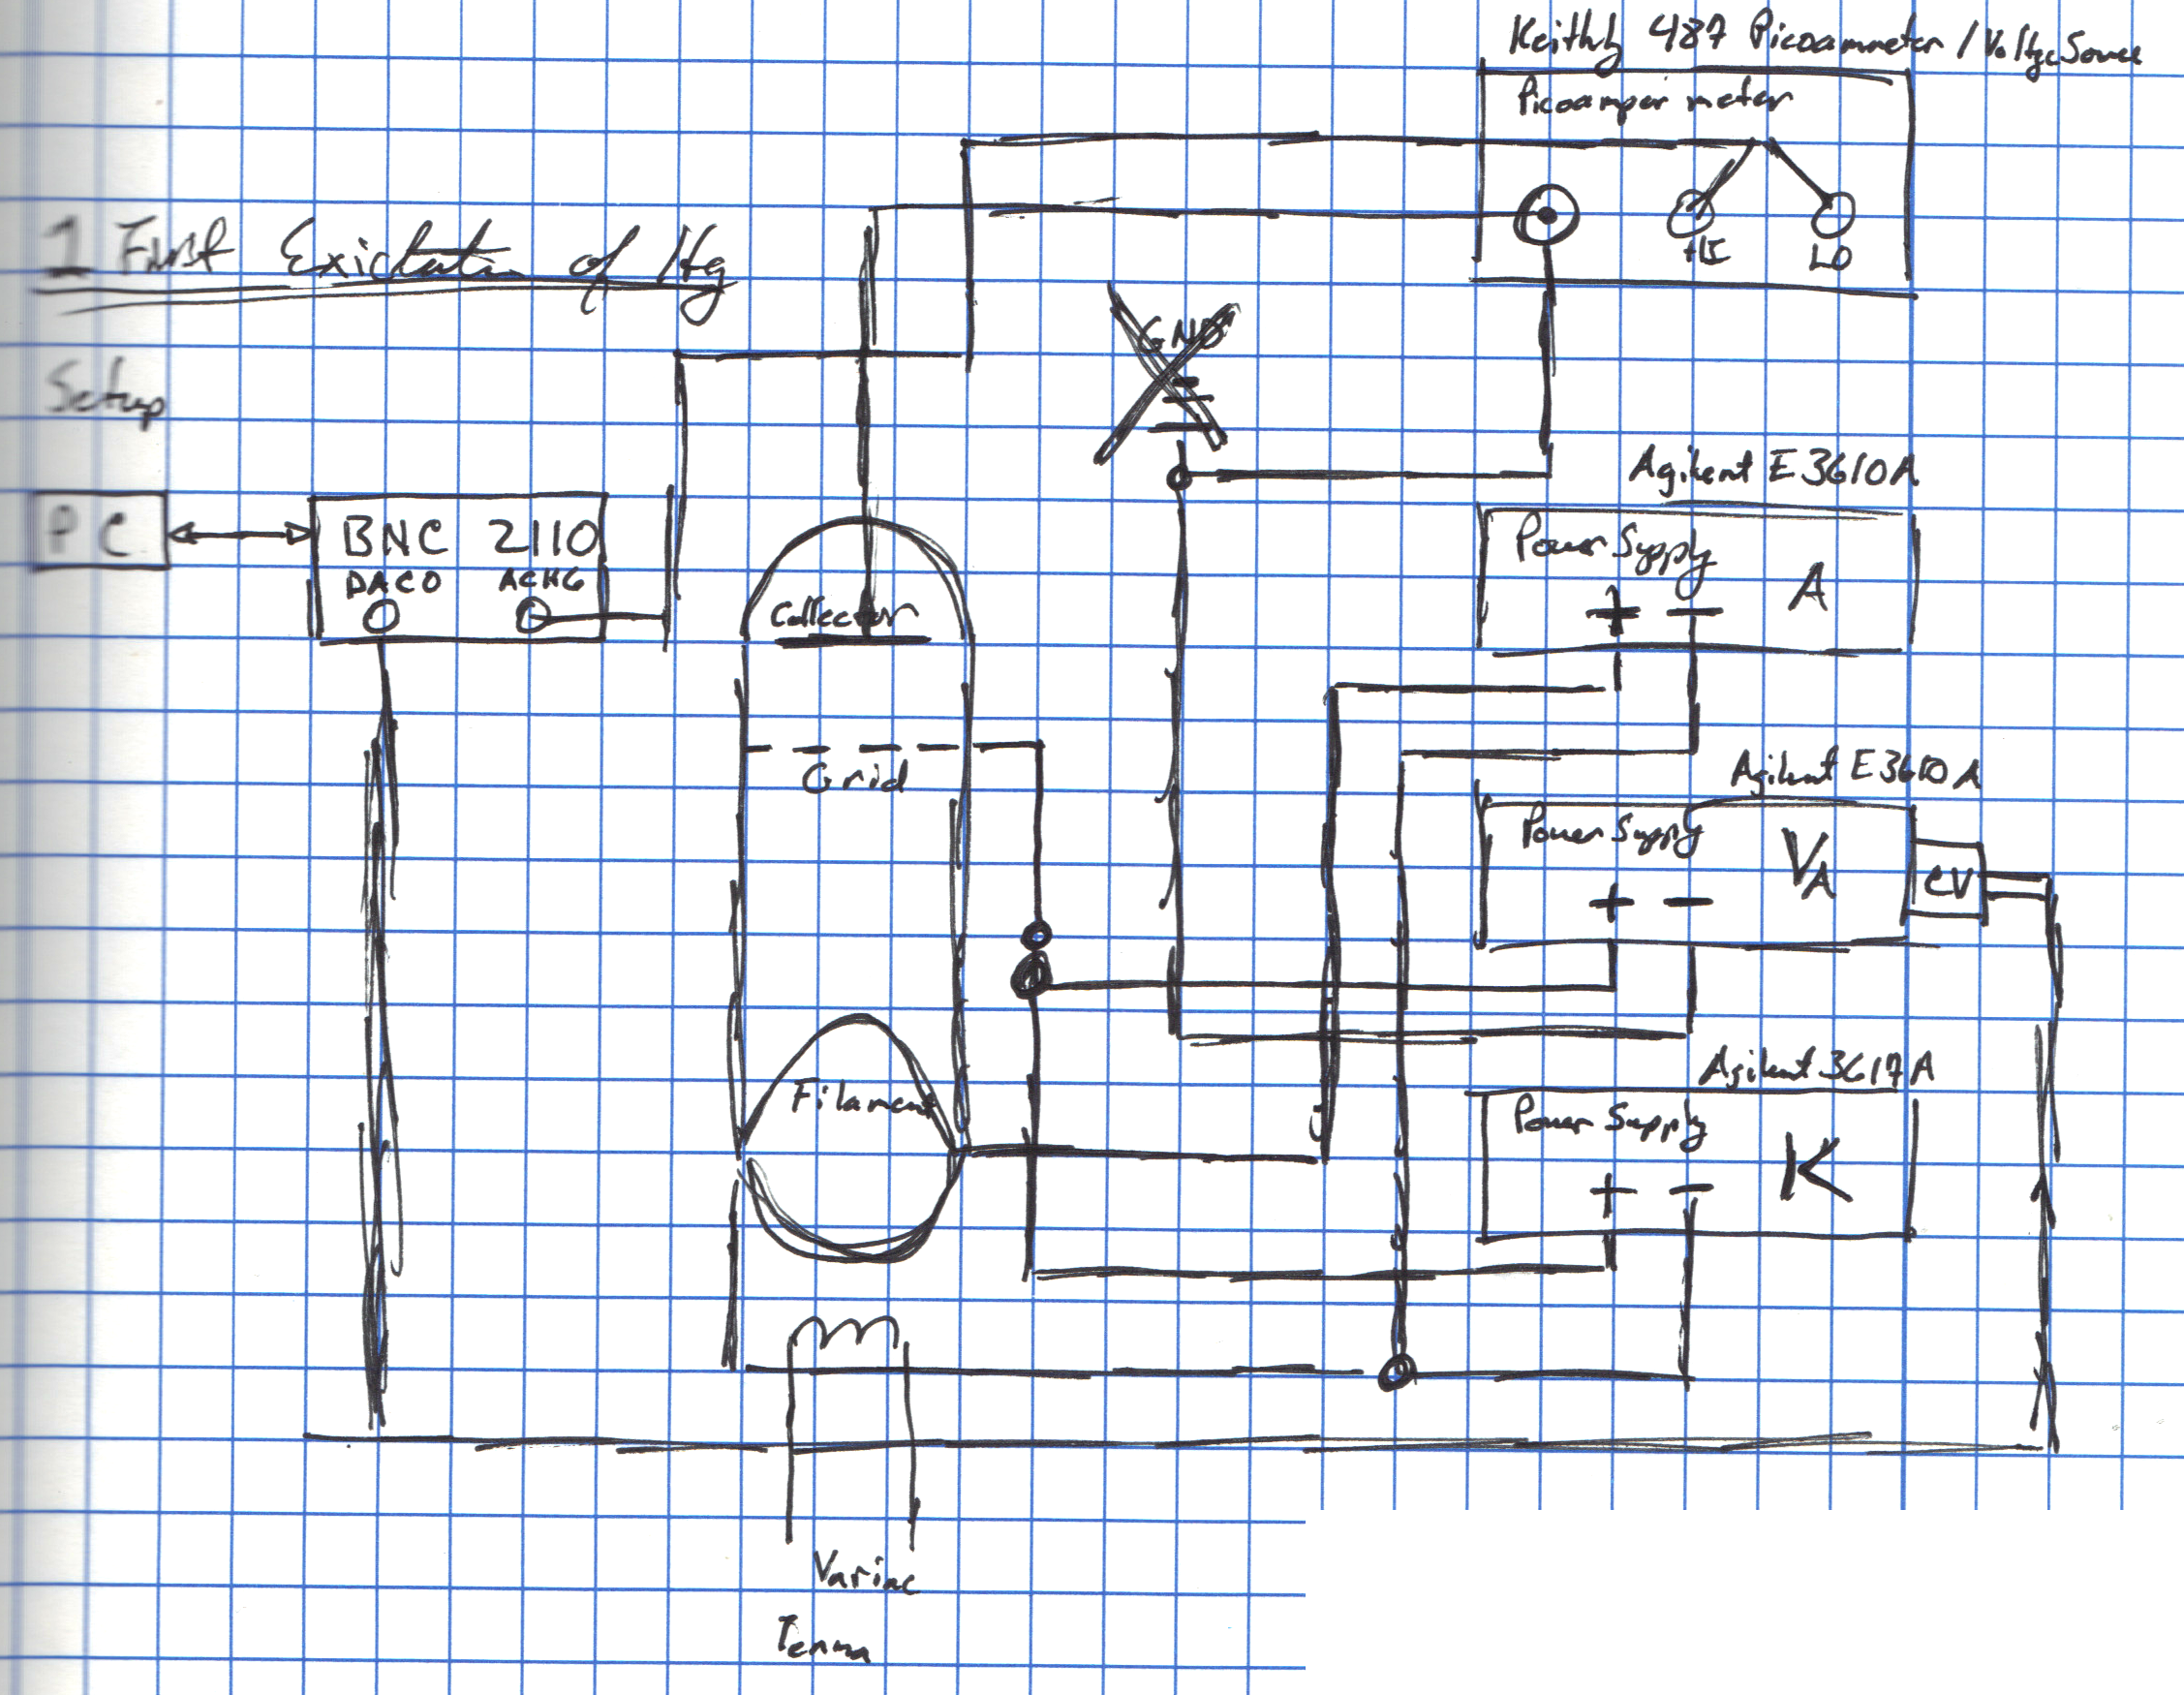
\includegraphics[width=3in]{images/HgSetup}
	\caption{Experimental setup as recorded in labratory notebook}
	\label{fig:HgSetup}
\end{figure}

A computer controlled Agilent 3617A power supply was connected to the filament and grid to provide the accelerating voltage. The collector plate was drawn to a Keithly 487 Picoammeter which measured the collected current and reported the results to a computer. A Tenma variac was connected to the vapor tube housing to heat the instrument.

\subsection{Procedure}

First the mercury vapor was heated to 180$^{\circ}$-200$^{\circ}$C using the variac. A thermocouple was inserted into the housing to monitor the temperature. When the temperature became stable, the retarding potential was set between 1.0 and 3.0V using the appropriate power supply. Similarly, the filament voltage was adjusted until the current through the filament wire was between 0.10-0.15A. The accelerating voltage power supply was turned on and set for PC control. The picoammeter was turned on and its autoscale feature disabled.

On the controlling PC, a Lab View program controlling the accelerating voltage power supply was opened. The program was then set to range the voltage from 0-55V in steps of 0.01V at a rate of 1ms/step. The program was executed and recorded collector current as a function of accelerating voltage. It is important to note that the Lab View program was not callibrated for the picoammeter, so collector current is measured in arbitrary units. The output filename and associated run parameters were also recorded.

\subsection{Results and Analysis}

Ten outputs of the program were recorded at a 0.01V step size, 1ms delay, 1.00V retarding potential and 0.10A filament current. For each of these runs, the polling rate of 1ms was fast enough to see 60Hz interference from the wall outlets. To compensate slightly for this, the data was smoothed using a running average over 64 points. The raw and smoothed data is displayed below in Fig. \ref{fig:HgData}.

\begin{figure}[h!]
	\centering
	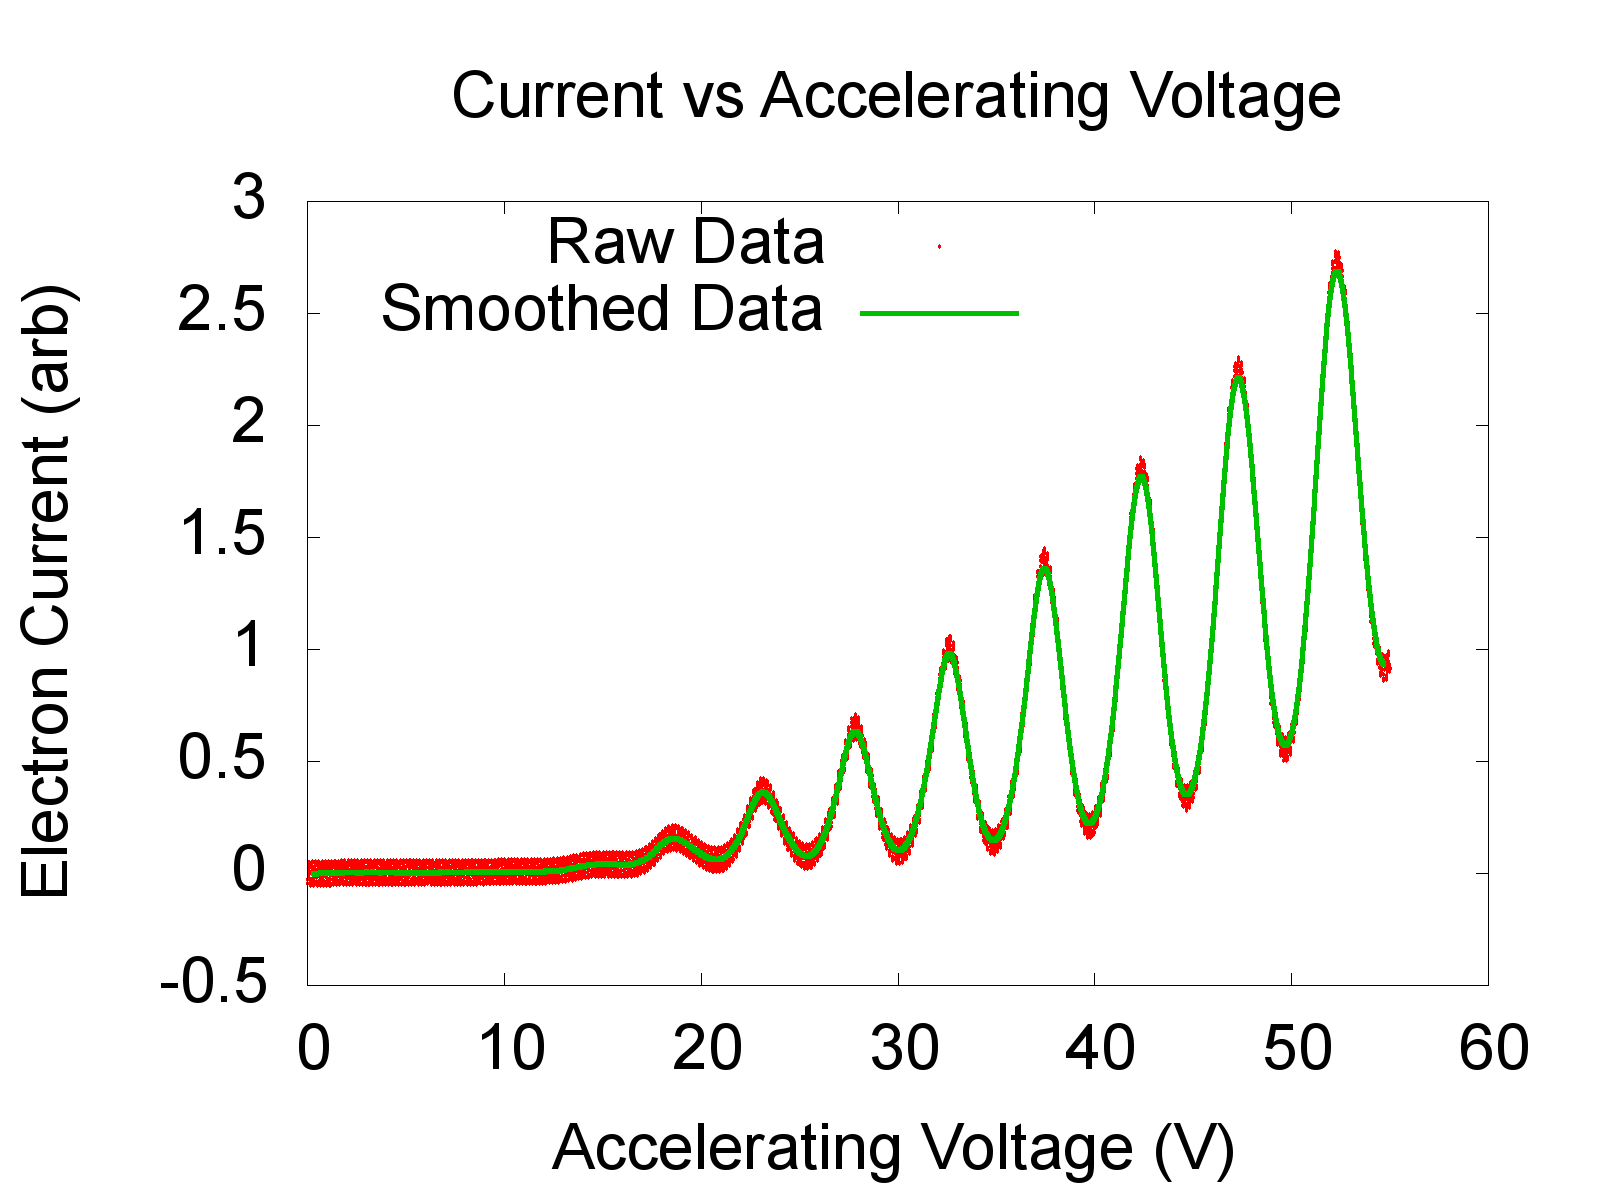
\includegraphics[width=3in]{images/Hg-smoothed}
	\caption{Collector current vs Accelerating voltage}
	\label{fig:HgData}
\end{figure}

Notice that the current increases as expected and undergoes sudden drops at regular intervals. At the first drop, electrons have just obtained enough energy to excite mercury once. The next drop allows an electon to excite two mercury atoms, and so on. As seen, the peaks of the graph at low accelerating voltages are not very well distinguished, so to measure the first excitation potential of mercury we will not take the first peak. Instead we will measure the average spacing between peaks.

The peak index and accelerating voltage were measured using a python script. This allows us to plot peak voltage vs peak index (n) as shown in Fig. \ref{fig:HgLine}. A linear regression is applied to this plot where the slope of the line represents the excitation energy per electron charge in V.

\begin{figure}[h!]
	\centering
	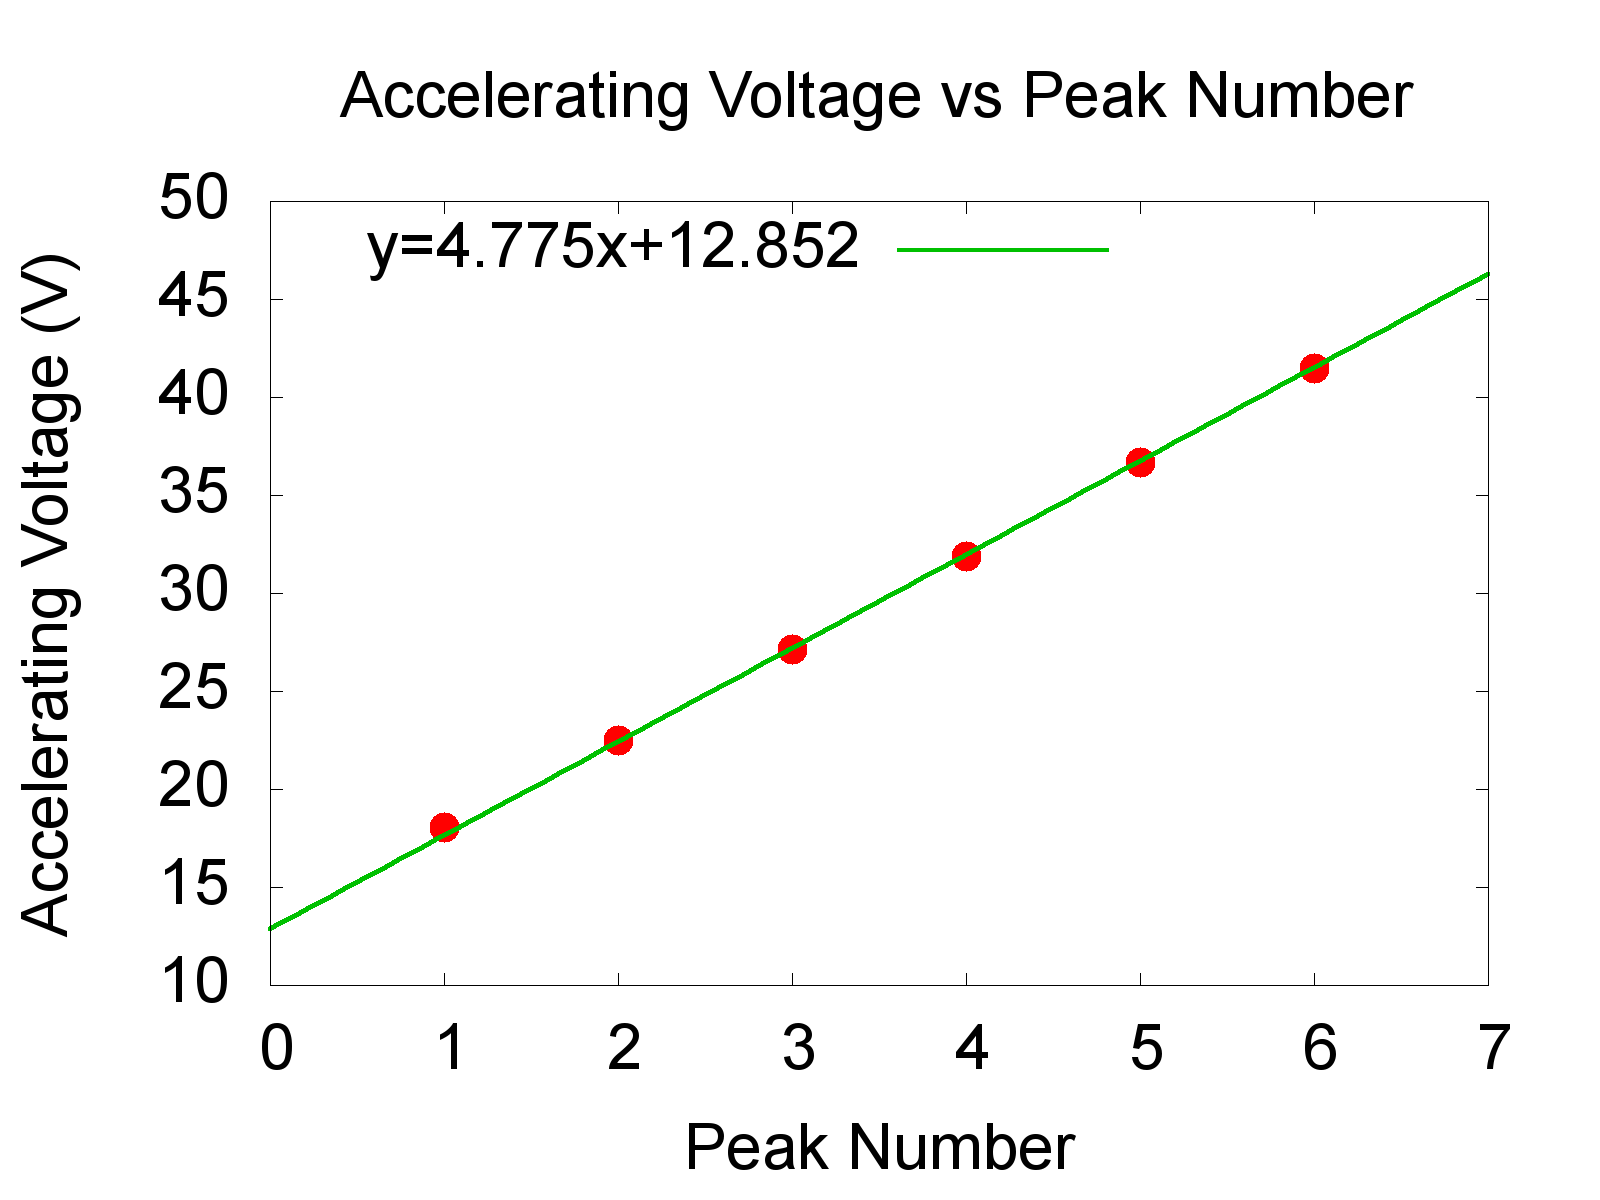
\includegraphics[width=3in]{images/HgLine}
	\caption{Peak Accelerating Voltage vs Peak Index}
	\label{fig:HgLine}
\end{figure}

In the example shown, we found the first excitation of mercury to be at 4.775eV. Repeating this for all runs and averaging, we found the first excitation of mercury to be 4.74eV with a standard deviation of 0.14eV.

%}}}

\section{Franck-Hertz Type Experiment with Helium}

\subsection{Equipment}


The expermiental setup, depicted in Fig. \ref{fig:HgSetup}, is very similar to the previous experiment. The mercury vapor has been replaced with a helium chamber and the retarding potential with a small 1.5V battery. The filament current is set with a power supply, accelerating voltage is computer controlled, and collector current measured. For Helium, there is no need to heat the sample before testing and the variac is removed.

\begin{figure}[h!]
	\centering
	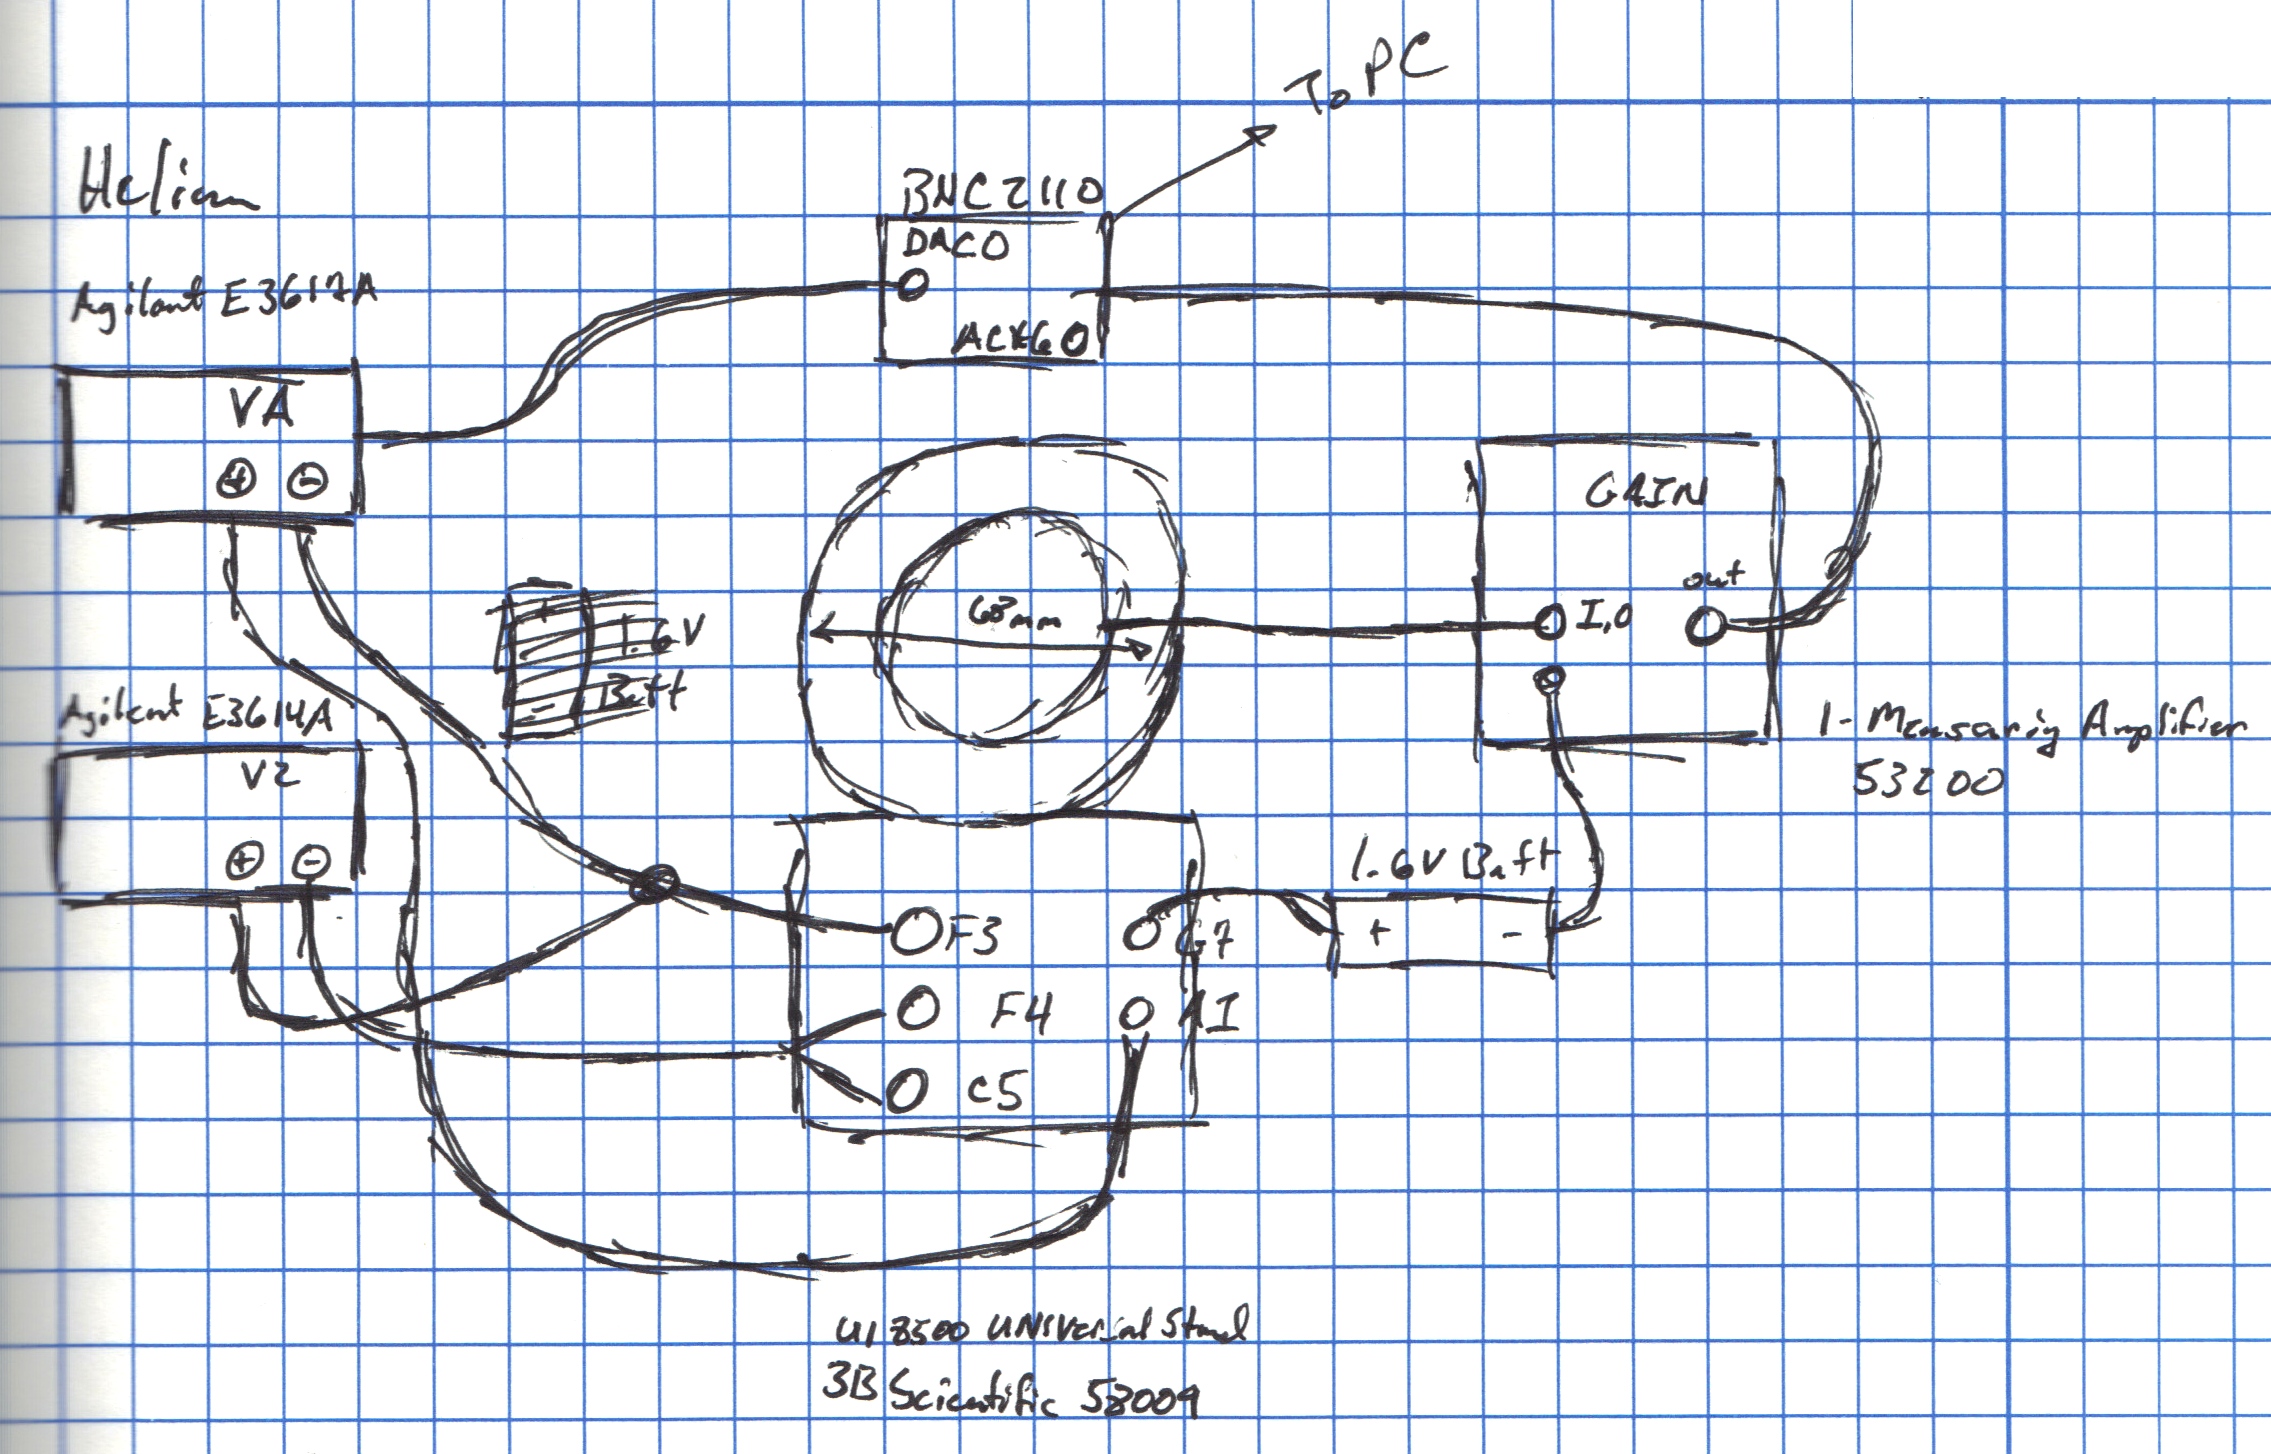
\includegraphics[width=3in]{images/HeliumSetup}
	\caption{Experimental setup as recorded in labratory notebook}
	\label{fig:HeSetup}
\end{figure}

\subsection{Procedure}

The filament current was set to 1.0A, then the Lab View program was opened. The accelerating voltage was instructed to vary from 0-25V in steps of .01V at a rate of 10ms/step. A slower rate is prefered in this experiment, to let the system reach equilibrium before measuring. The resulting collector current vs accelerating voltages were saved in output files with their respective settings. A total of 10 runs were performed.

\subsection{Results and Analysis}

As with the mercury experiment, the data collected contained high noise and was smoothed under the same algorithm as shown in Fig. \ref{fig:HeData}.

\begin{figure}[h!]
	\centering
	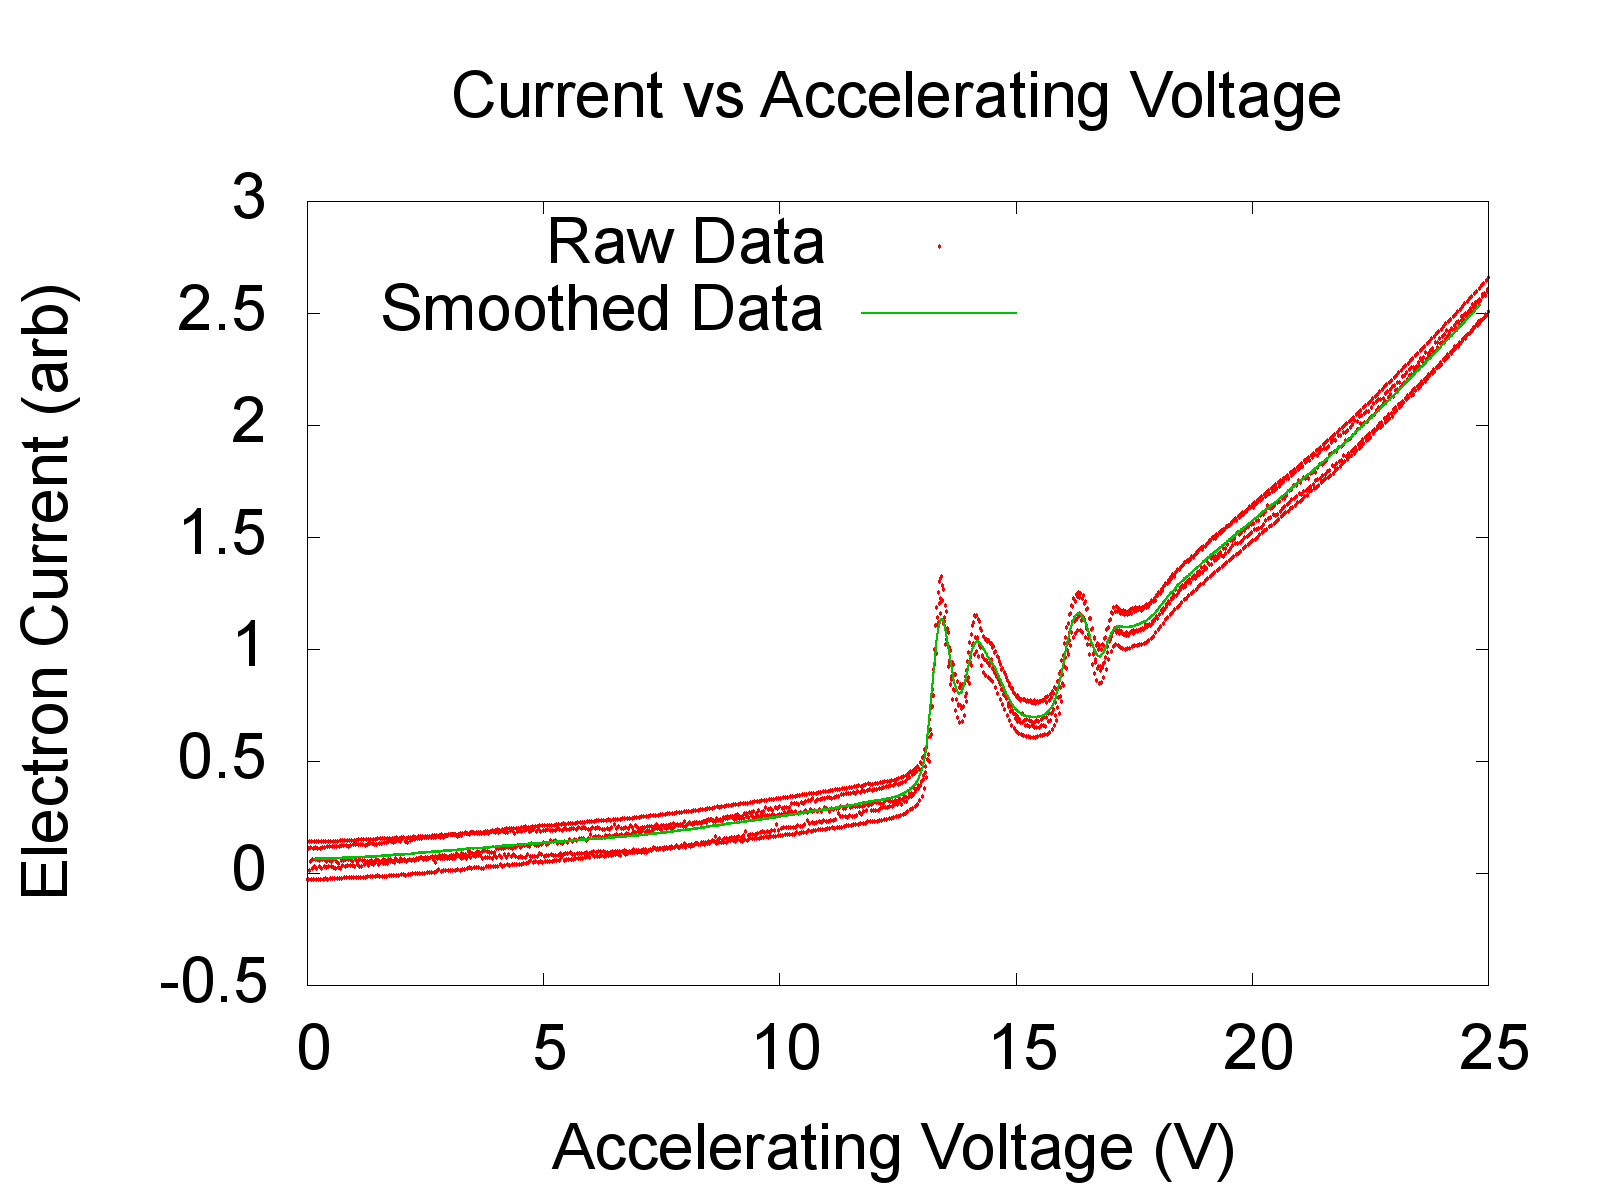
\includegraphics[width=3in]{images/He-smoothed}
	\caption{Collector current vs Accelerating voltage}
	\label{fig:HeData}
\end{figure}

Notice that Helium does not show the well defined recurring pattern that is evident in mercury. Instead, we find collector current increases abruptly when excitations first begin at the first marked point in Fig. \ref{fig:HeMark}. The spacing of energies in Helium allows for excitations to increase collector current, however at higher energies the electrons are not captured as often. Thus the curve falls. Each new minimum in the graph represents the start of an excited state. At some point, the electron gun begins to ionize Helium causing monotonic increase in current and masks the quantization.

\begin{figure}[h!]
	\centering
	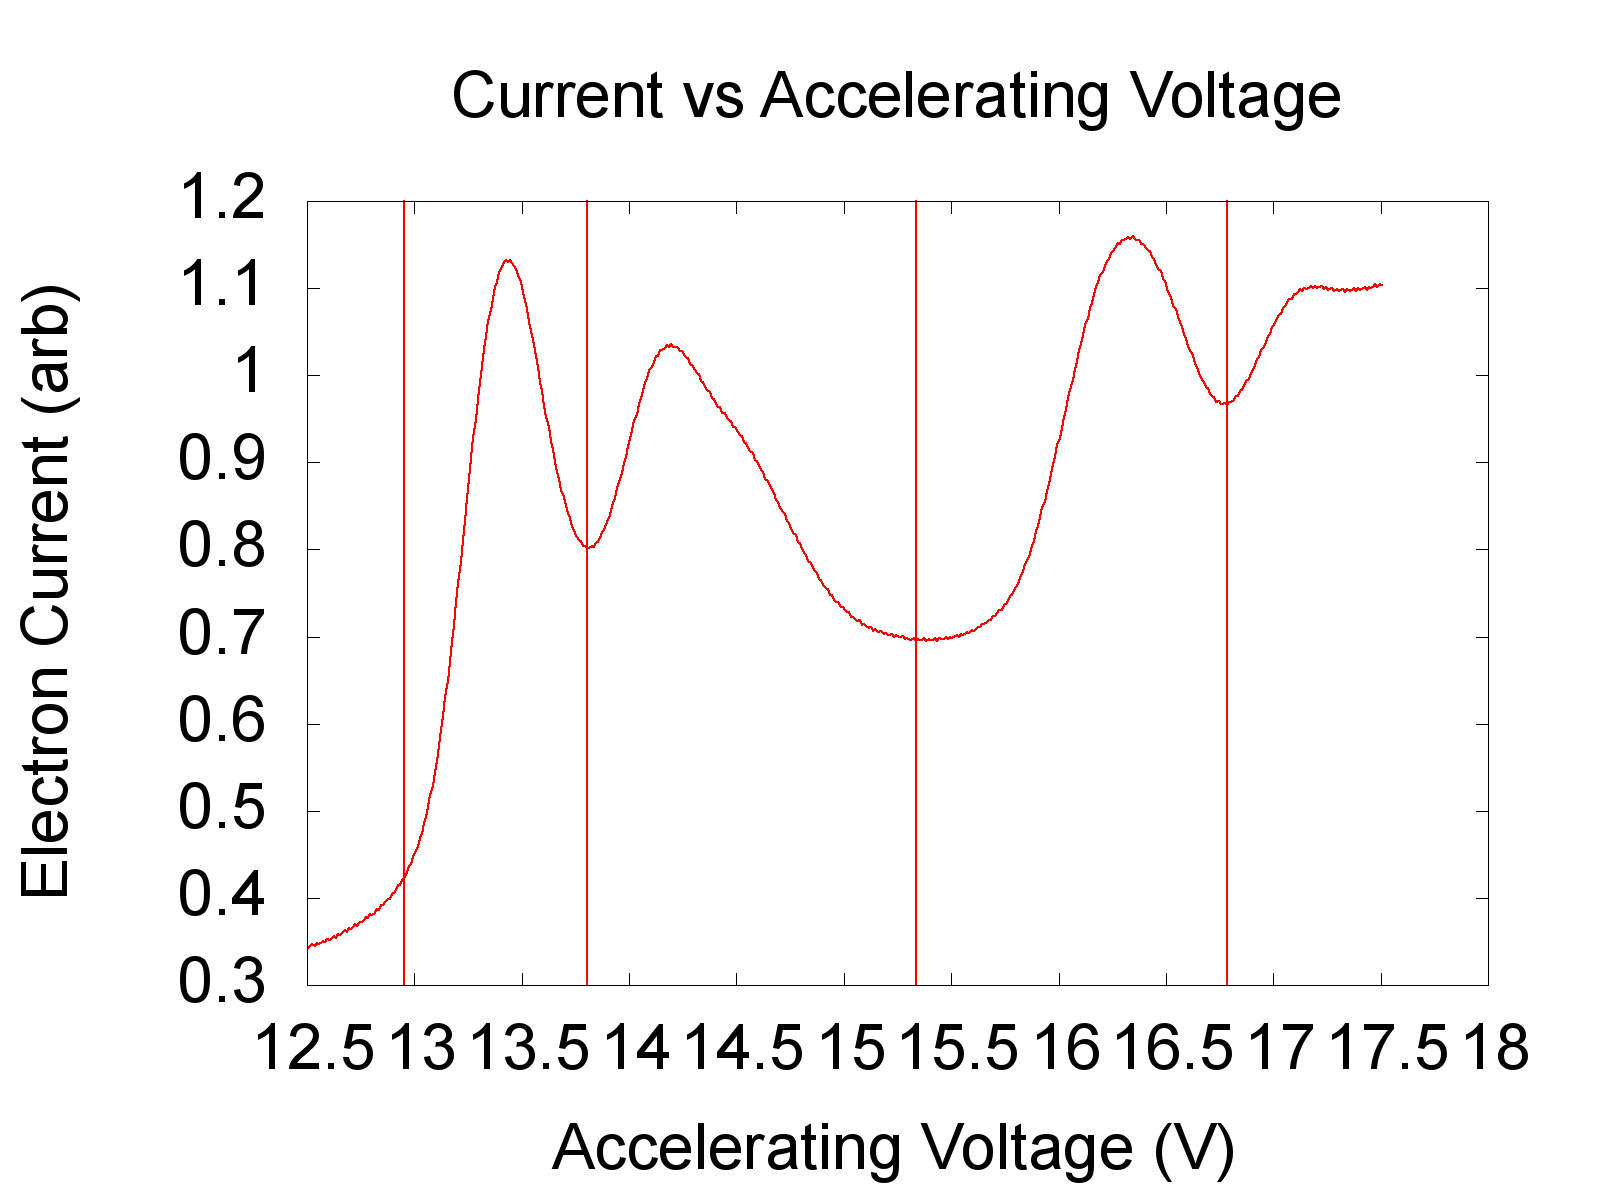
\includegraphics[width=3in]{images/HeMark}
	\caption{Collector current vs Accelerating voltage with marked minimums}
	\label{fig:HeMark}
\end{figure}

Over ten runs, we found the first increase to be at 13.8eV$\pm$0.6eV, and the next three minima at 15.0$\pm$0.3eV, 16.5$\pm$0.25, 18.0$\pm$0.3eV. While these values cannot be interpreted directly as the excitation energies of Helium due to the apparatus constraints, we can see that the spacing is not uniform. With a shift by 6eV, these values align very well with the 1s2s,1s2p,1s3s, and 1s5s energy levels of Helium at 19.8, 21.0, 22.7, and 24.0eV. This implies that we are witnessing multiple different energy levels instead of single excitations as with mercury.

\section{Visual Observations of He and Na}

\subsection{Equipment}

A sodium vapor and Helium vapor lamp are directed into a collimator. The collimator directs the light into a Welsch scientific diffraction grating, rated at 15,000 lines/in, which splits the beam. A freely rotating eye piece is used to view the diffracted beam. The collimator, diffraction grating, platform, and telescope are part of a American Optical Company spectroscope and displayed in Fig. \ref{fig:spectroscope}.

\begin{figure}[h!]
	\centering
	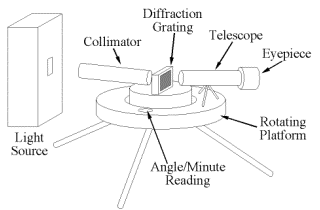
\includegraphics[width=3in]{images/spectroscope}
	\caption{Spectrum Observing Apparatus}
	\label{fig:spectroscope}
\end{figure}

\subsection{Procedure}
Turn on the sodium lamp and allow it to heat. When it turned yellow, measurements continued. The eyepiece was aligned with the undiffracted beam, and the telescope angle recorded as $\phi_{0}=213^{\circ}43'$. Subsequent measurements are recorded as marked on the spectroscope, but taken in reference to the undiffracted angle.

To measure an angle, the viewpiece is aligned with a spectrum line using the telescope crosshair. Then the telescope is locked in place and a fine adjustment knob is used to better align the telescope. The telescope angle is then read from the spectroscope.

\subsection{Results}

To measure the diffraction grating spacing, we used the sodium lamp and located the sodium d-line to the left and right of $\phi_{0}$ and recorded these as $\phi_{L}=234^{\circ}33'$ and $\phi_{R}=192^{\circ}55'$. Then the diffraction spacing $d$ was calculated using:

\begin{equation}
	\label{eq:ld}
	\frac{1}{2}\left(\sin\theta_{R}+\sin\theta_{L}\right)=\frac{m\lambda}{d}
\end{equation}

Using the measured values and taking $m=1, \lambda=5893\AA$, we found $d=1.6\mu m\pm 0.1\mu m$ in agreement with the rated value of $1.69\mu m$.

Next we measured the splitting of the sodium d-line. However, the diffraction grating did not separate the lines far enough to be clearly distinct. Instead we saw one band with three regions in a weak-strong-weak pattern. We took the rightmost edge of the band as the location of the first line and the rightmost edge of the strong region to be the location of the second line. We measured an angular separation $\Delta\theta=1.2\cdot10^{-3}$ radians. Using the equation below, we found the line splitting in wavelength to be $\Delta\lambda=7.7\pm1\AA$. This is near to the expected value of $5.97\AA$; however, our result cannot match the precision due to instrument limitations.

\begin{equation}
	\Delta\lambda=\frac{d}{m}\cos\theta \Delta\theta
\end{equation}

Finally we replaced the sodium lamp with the Helium lamp and recorded every observable line. Using Eq. \ref{eq:ld}, we calculated the associated wavelength of the emission and compared with known values from NIST\cite{NIST} as shown in Table \ref{tb:he}. Note angles are listed in degrees and wavelenghts given in angstroms. $\lambda_{e}$ represents the experimental or calculated wavelength while $\lambda_{t}$ is the theoretical.

\begin{table}[h!]
	\label{tb:he}
	\caption{Observed emissions and estimated transitions}
	\begin{tabular}{|c|c|c|c|c|}
		\hline
		Transition & $\theta_{R}$ & $\theta_{L}$ & $\lambda_{e}$ & $\lambda_{t}$ \\ \hline
		1s2p$\rightarrow$1s4d$^{1}$ & 15.67 & 15.72 & 4485 & 4471 \\ 
		1s2p$\rightarrow$1s4s$^{1}$ & 16.55 & 16.55 & 4724 & 4713 \\ 
		1s2p$^{2}\rightarrow$1s4d$^{1}$ & 17.28 & 17.27 & 4924 & 4922 \\ 
		1s2s$^{1}\rightarrow$1s3p & 17.72 & 17.63 & 5035 & 5016 \\ 
		1s2p$\rightarrow$1s3d & 20.78 & 20.78 & 5884 & 5876 \\ 
		1s2p$^{2}\rightarrow$1s3d & 23.78 & 24.22 & 6745 & 6678 \\ 
		1s2p$\rightarrow$1s3s & 25.28 & 25.22 & 7073 & 7065 \\ 
		\hline
	\end{tabular}
\end{table}

\nocite{*}
\bibliography{references}
\bibliographystyle{plain}
\end{document}
